\documentclass[12pt,a4paper]{article}
\usepackage{ctex}
\usepackage{geometry}
\usepackage{graphicx}
\usepackage{setspace}
\usepackage{listings}
\usepackage{listingsutf8}
\usepackage{xcolor}
\usepackage{float} 
\usepackage[colorlinks=true,linkcolor=blue]{hyperref}

\geometry{left=3cm,right=3cm,top=2.5cm,bottom=2.5cm}

% 代码样式
\lstset{
    language=Java,
    inputencoding=utf8,
    basicstyle=\ttfamily\small,
    keywordstyle=\color{blue}\bfseries,
    commentstyle=\color{green!50!black},
    stringstyle=\color{orange},
    showstringspaces=false,
    numbers=left,
    numberstyle=\tiny,
    breaklines=true,
    frame=single
}

\begin{document}

% ================= 封面 =================
\begin{titlepage}
\centering

% 校徽 Logo 
\makebox[\textwidth][c]{%
  
\includegraphics[height=4cm]{fengmian.png}%
}
\vspace*{2cm}

% 学院名称
{\zihao{1}\heiti 信息科学与工程学院}\\[1cm]

% 学年学期
{\zihao{4} 2025---2026 \kaishu学年第一学期}\\[1.5cm]

% 报告标题
\makebox[\textwidth][c]{%
  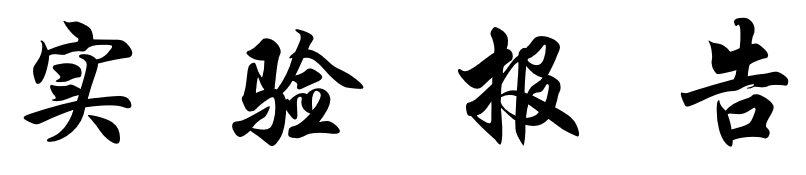
\includegraphics[height=2cm]{shiyanbaogao.png}%
}
\\[2em] % 空行
% 实验基本信息表
\zihao{4} 
\renewcommand{\arraystretch}{1.8} % 表格行距
\begin{tabular}{rl}
\heiti 课程名称: & \underline{\makebox[18em][c]{\fangsong Java 编程技术}} \\
\vspace{1cm}
\heiti 实验名称: & \underline{\makebox[18em][c]{\fangsong 第四次实验}} \\
\kaishu 专  业  班  级 & \underline{\makebox[18em][c]{\kaishu 通信一班}} \\
\kaishu 学  生  学  号 & \underline{\makebox[18em][c]{\kaishu 202300120317}} \\
\kaishu 学  生  姓  名 & \underline{\makebox[18em][c]{\kaishu 陈都阳}} \\
\kaishu 实  验  时  间 & \underline{\makebox[18em][c]{\kaishu 2025年10月16日}} \\
\end{tabular}

\vfill
\end{titlepage}

% ================= 正文 =================
\section*{【实验目的】}
\begin{enumerate}
    \item 掌握抽象类 (\texttt{abstract class}) 与抽象方法 (\texttt{abstract method}) 的定义与使用。
    \item 理解成员变量的继承与隐藏、方法的重载与覆盖之间的区别。
    \item 深入理解 \texttt{this}、\texttt{super} 与 \texttt{static} 关键字在类设计中的作用与限制。
    \item 掌握接口 (\texttt{interface}) 与继承的综合应用,理解接口回调机制。
    \item 学习 Java 反射机制 (\texttt{Reflection}) 的基本思想及其动态加载原理。
    \item 通过综合实验(\texttt{Car}、\texttt{Plane} 等类)熟悉类的动态加载与扩展性设计。
\end{enumerate}

\section*{【实验要求】}
\begin{enumerate}
    \item 按实验内容要求完成各部分程序设计,代码中需包含必要注释,命名规范清晰。
    \item 编译运行程序,并截图保存实验结果,写明实验思路与运行分析。
    \item 在实验报告中对核心代码进行分析说明,阐述抽象类、继承、接口与反射机制的理解。
    \item 撰写实验心得,反思实验中遇到的问题及解决方法,可总结有价值的资料与经验。
    \item 程序应可在命令行下运行(如:\texttt{java ComputeTime Car 10 20 30}),计算结果保留两位小数。
\end{enumerate}

\section*{【第一个实验具体内容】}
代码框在不同平台上兼容的问题,代码部分的注释翻译成英文了,原版代码请查看代码支撑材料。
\subsection*{流程图}

\begin{figure}[H]
\centering
\includegraphics[width=0.8\textwidth]{oneb1.png}
\caption{流程图}
\end{figure}

\subsection*{源代码说明}
该程序定义抽象类 Shape,并由 Rectangle 与 Circle 实现 area() 与 printArea() 方法以计算并打印图形面积。构造器用于初始化尺寸,子类重写具体计算逻辑。主程序创建示例对象并调用打印方法以输出矩形和圆的面积;点击查看\hyperref[sec:one]{One.java完整代码}。

\subsection*{实验过程与结果}

\begin{figure}[H]
\centering
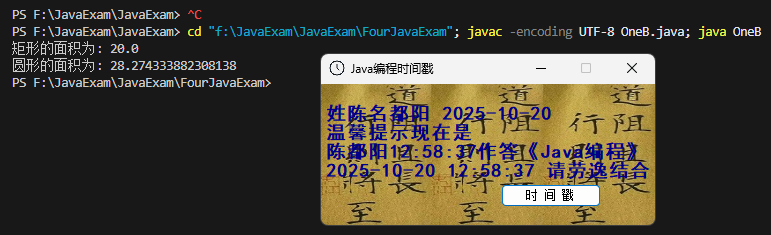
\includegraphics[width=0.8\textwidth]{oneb.png}
\caption{运行结果}
\end{figure}

\section*{【第二个实验具体内容】}
\subsection*{流程图}

\begin{figure}[H]
\centering
\includegraphics[width=0.8\textwidth]{twob1.png}
\caption{流程图}
\end{figure}

\subsection*{源代码说明}
演示继承、方法覆盖与重载的基本使用。类 A 提供 sum1() 与 sum2(int) 等方法,子类 B 覆盖无参 sum2() 并重载 sum2(int),同时提供 sum3() 调用父类实现。主程序实例化子类并调用这些方法以验证覆盖、重载与 super 的行为;点击查看\hyperref[sec:two]{Two.java完整代码}。

\subsection*{实验过程与结果}

\begin{figure}[H]
\centering
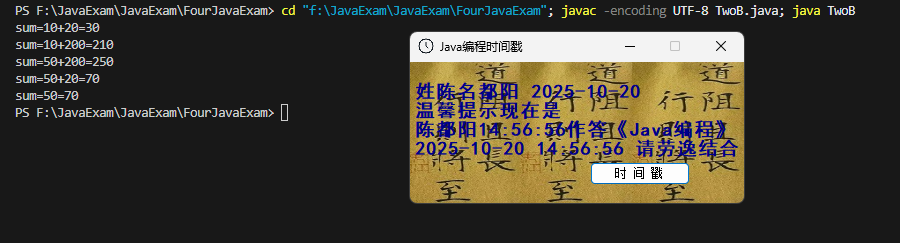
\includegraphics[width=0.8\textwidth]{twob.png}
\caption{运行结果}
\end{figure}

\section*{【第三个实验具体内容】}
\subsection*{流程图}

\begin{figure}[H]
\centering
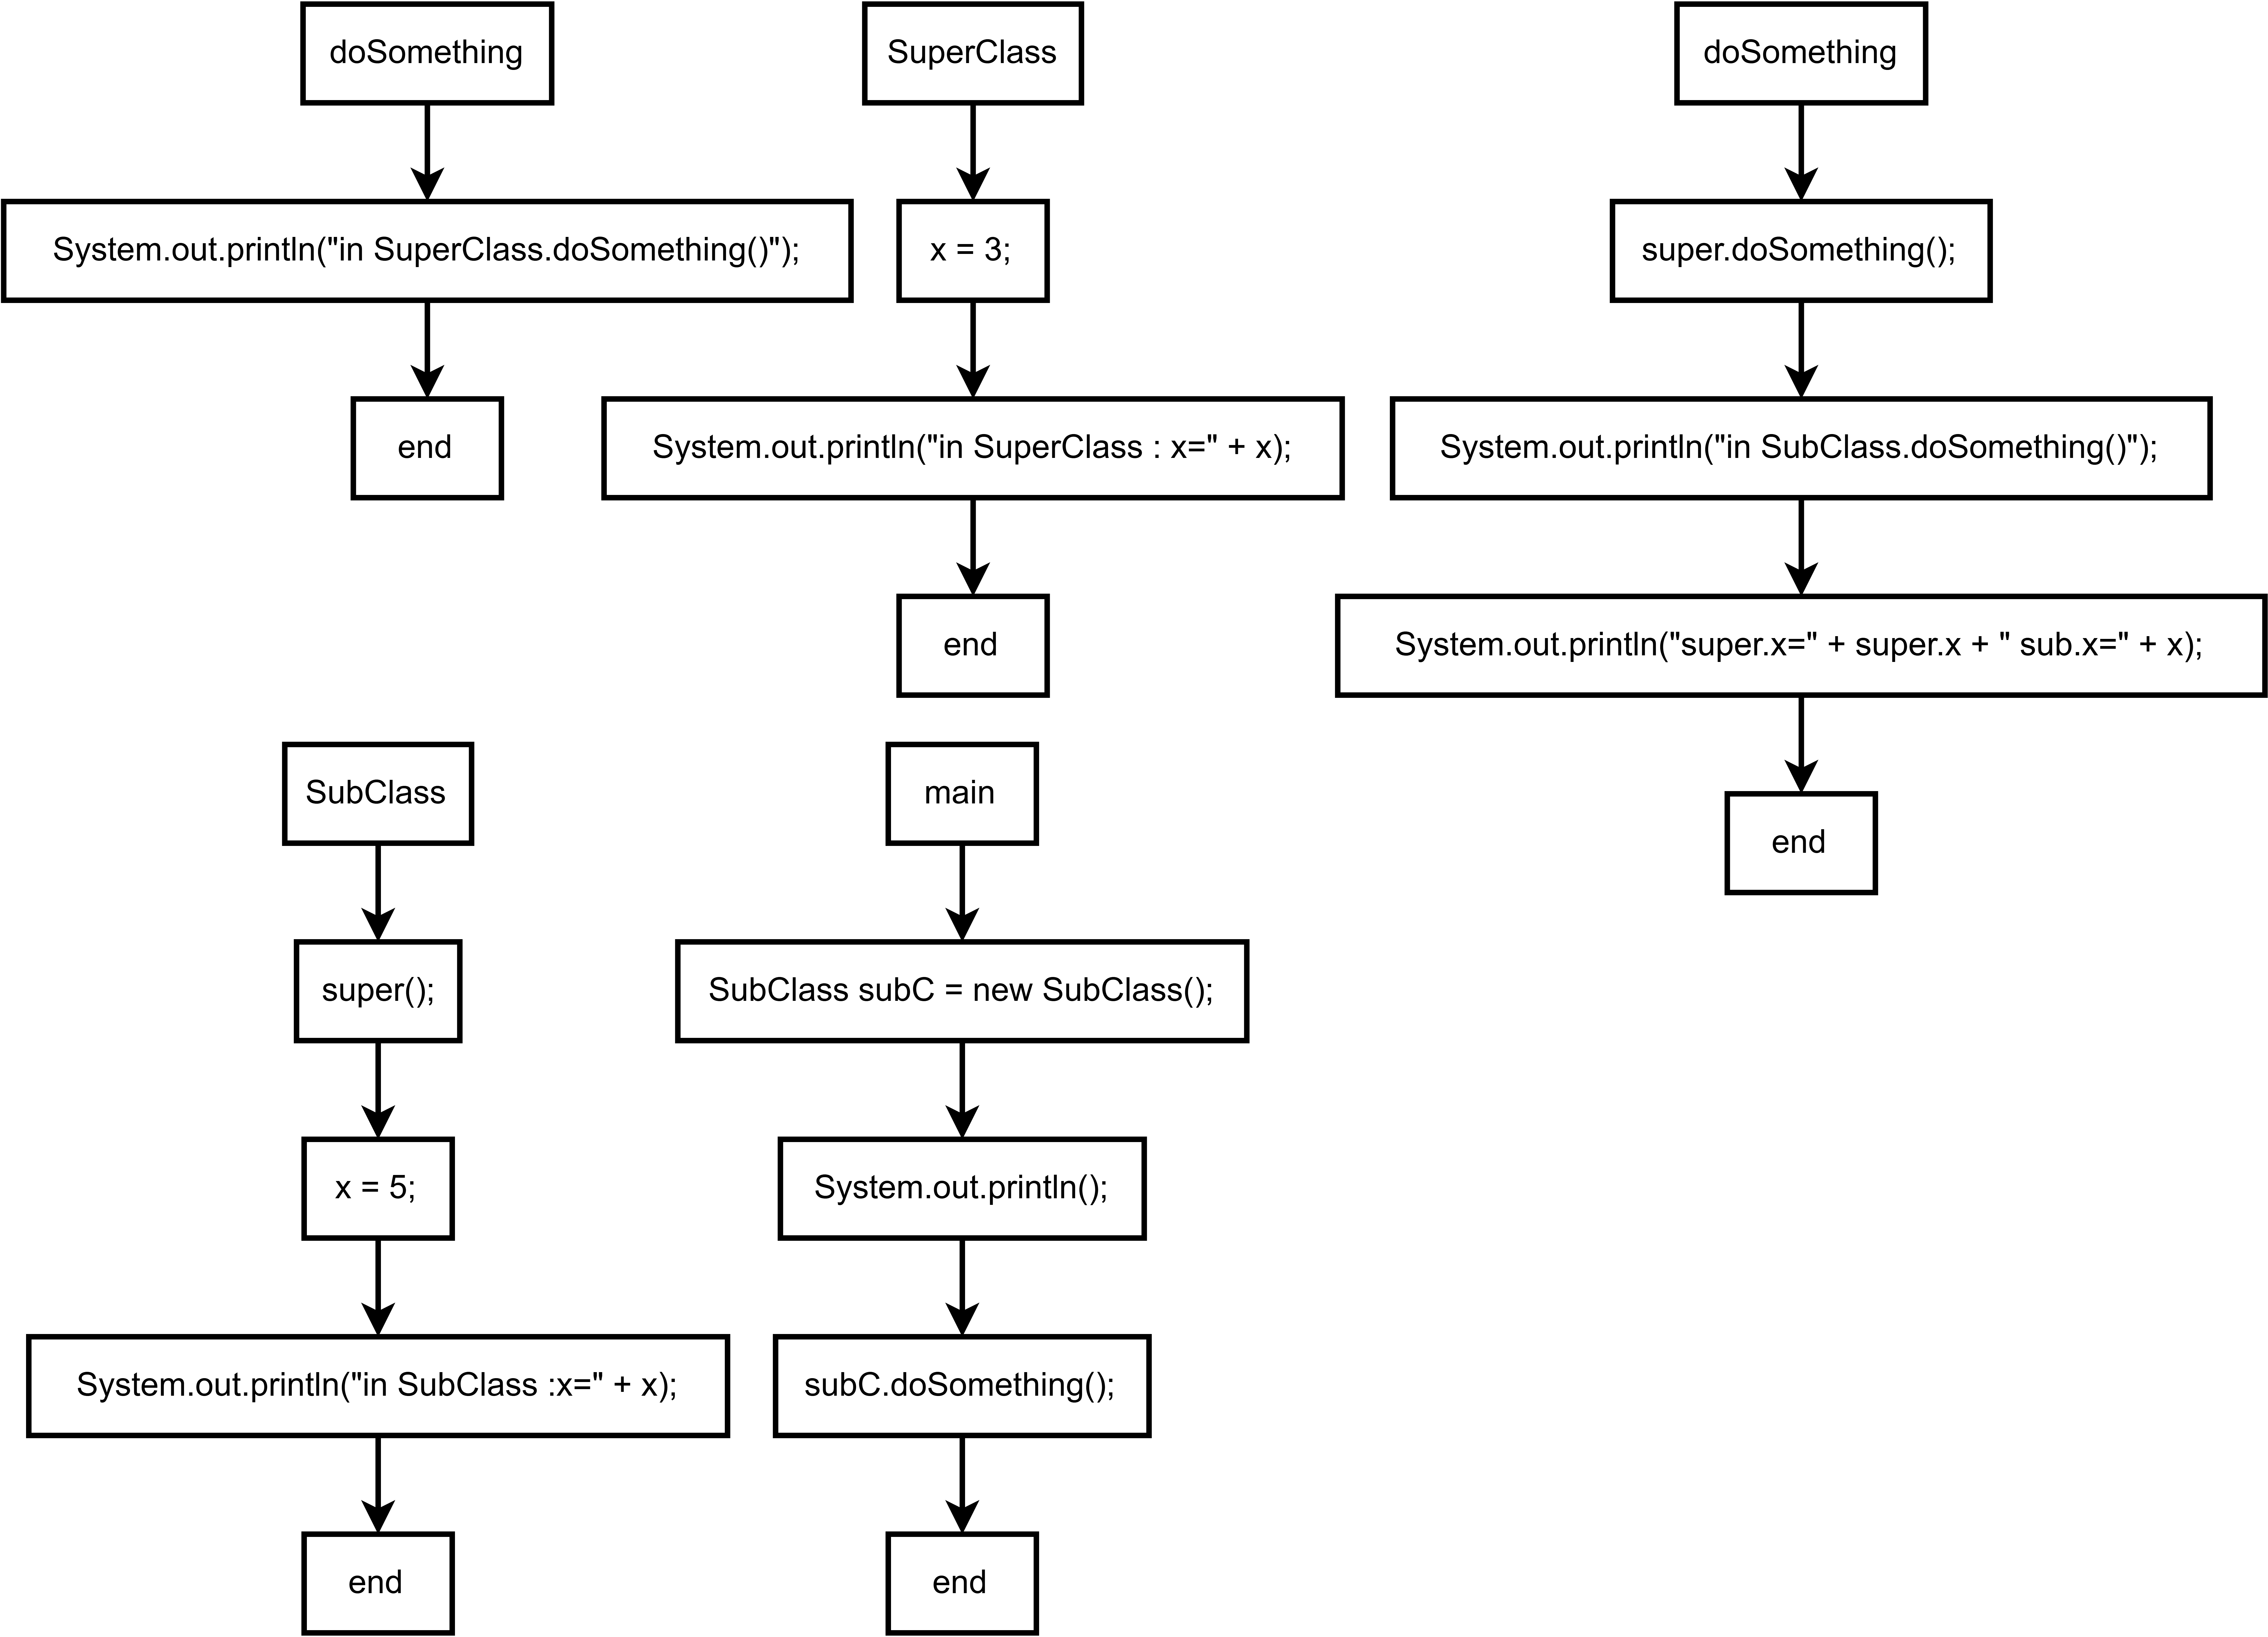
\includegraphics[width=0.8\textwidth]{threeb1.png}
\caption{流程图}
\end{figure}

\subsection*{源代码说明}
展示父类与子类构造器调用及方法重写的行为。SuperClass 在构造器中初始化字段并打印,SubClass 调用 super() 并覆盖 doSomething(),示例中同时输出 super.x 与子类字段以比较作用域。主程序创建子类实例并调用方法以观察构造与方法执行顺序;点击查看\hyperref[sec:three]{Three.java完整代码}。

\subsection*{实验过程与结果}

\begin{figure}[H]
\centering
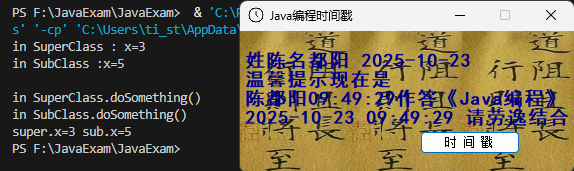
\includegraphics[width=0.8\textwidth]{threeb.png}
\caption{运行结果}
\end{figure}

\section*{【第四个实验具体内容】}
\subsection*{流程图}

\begin{figure}[H]
\centering
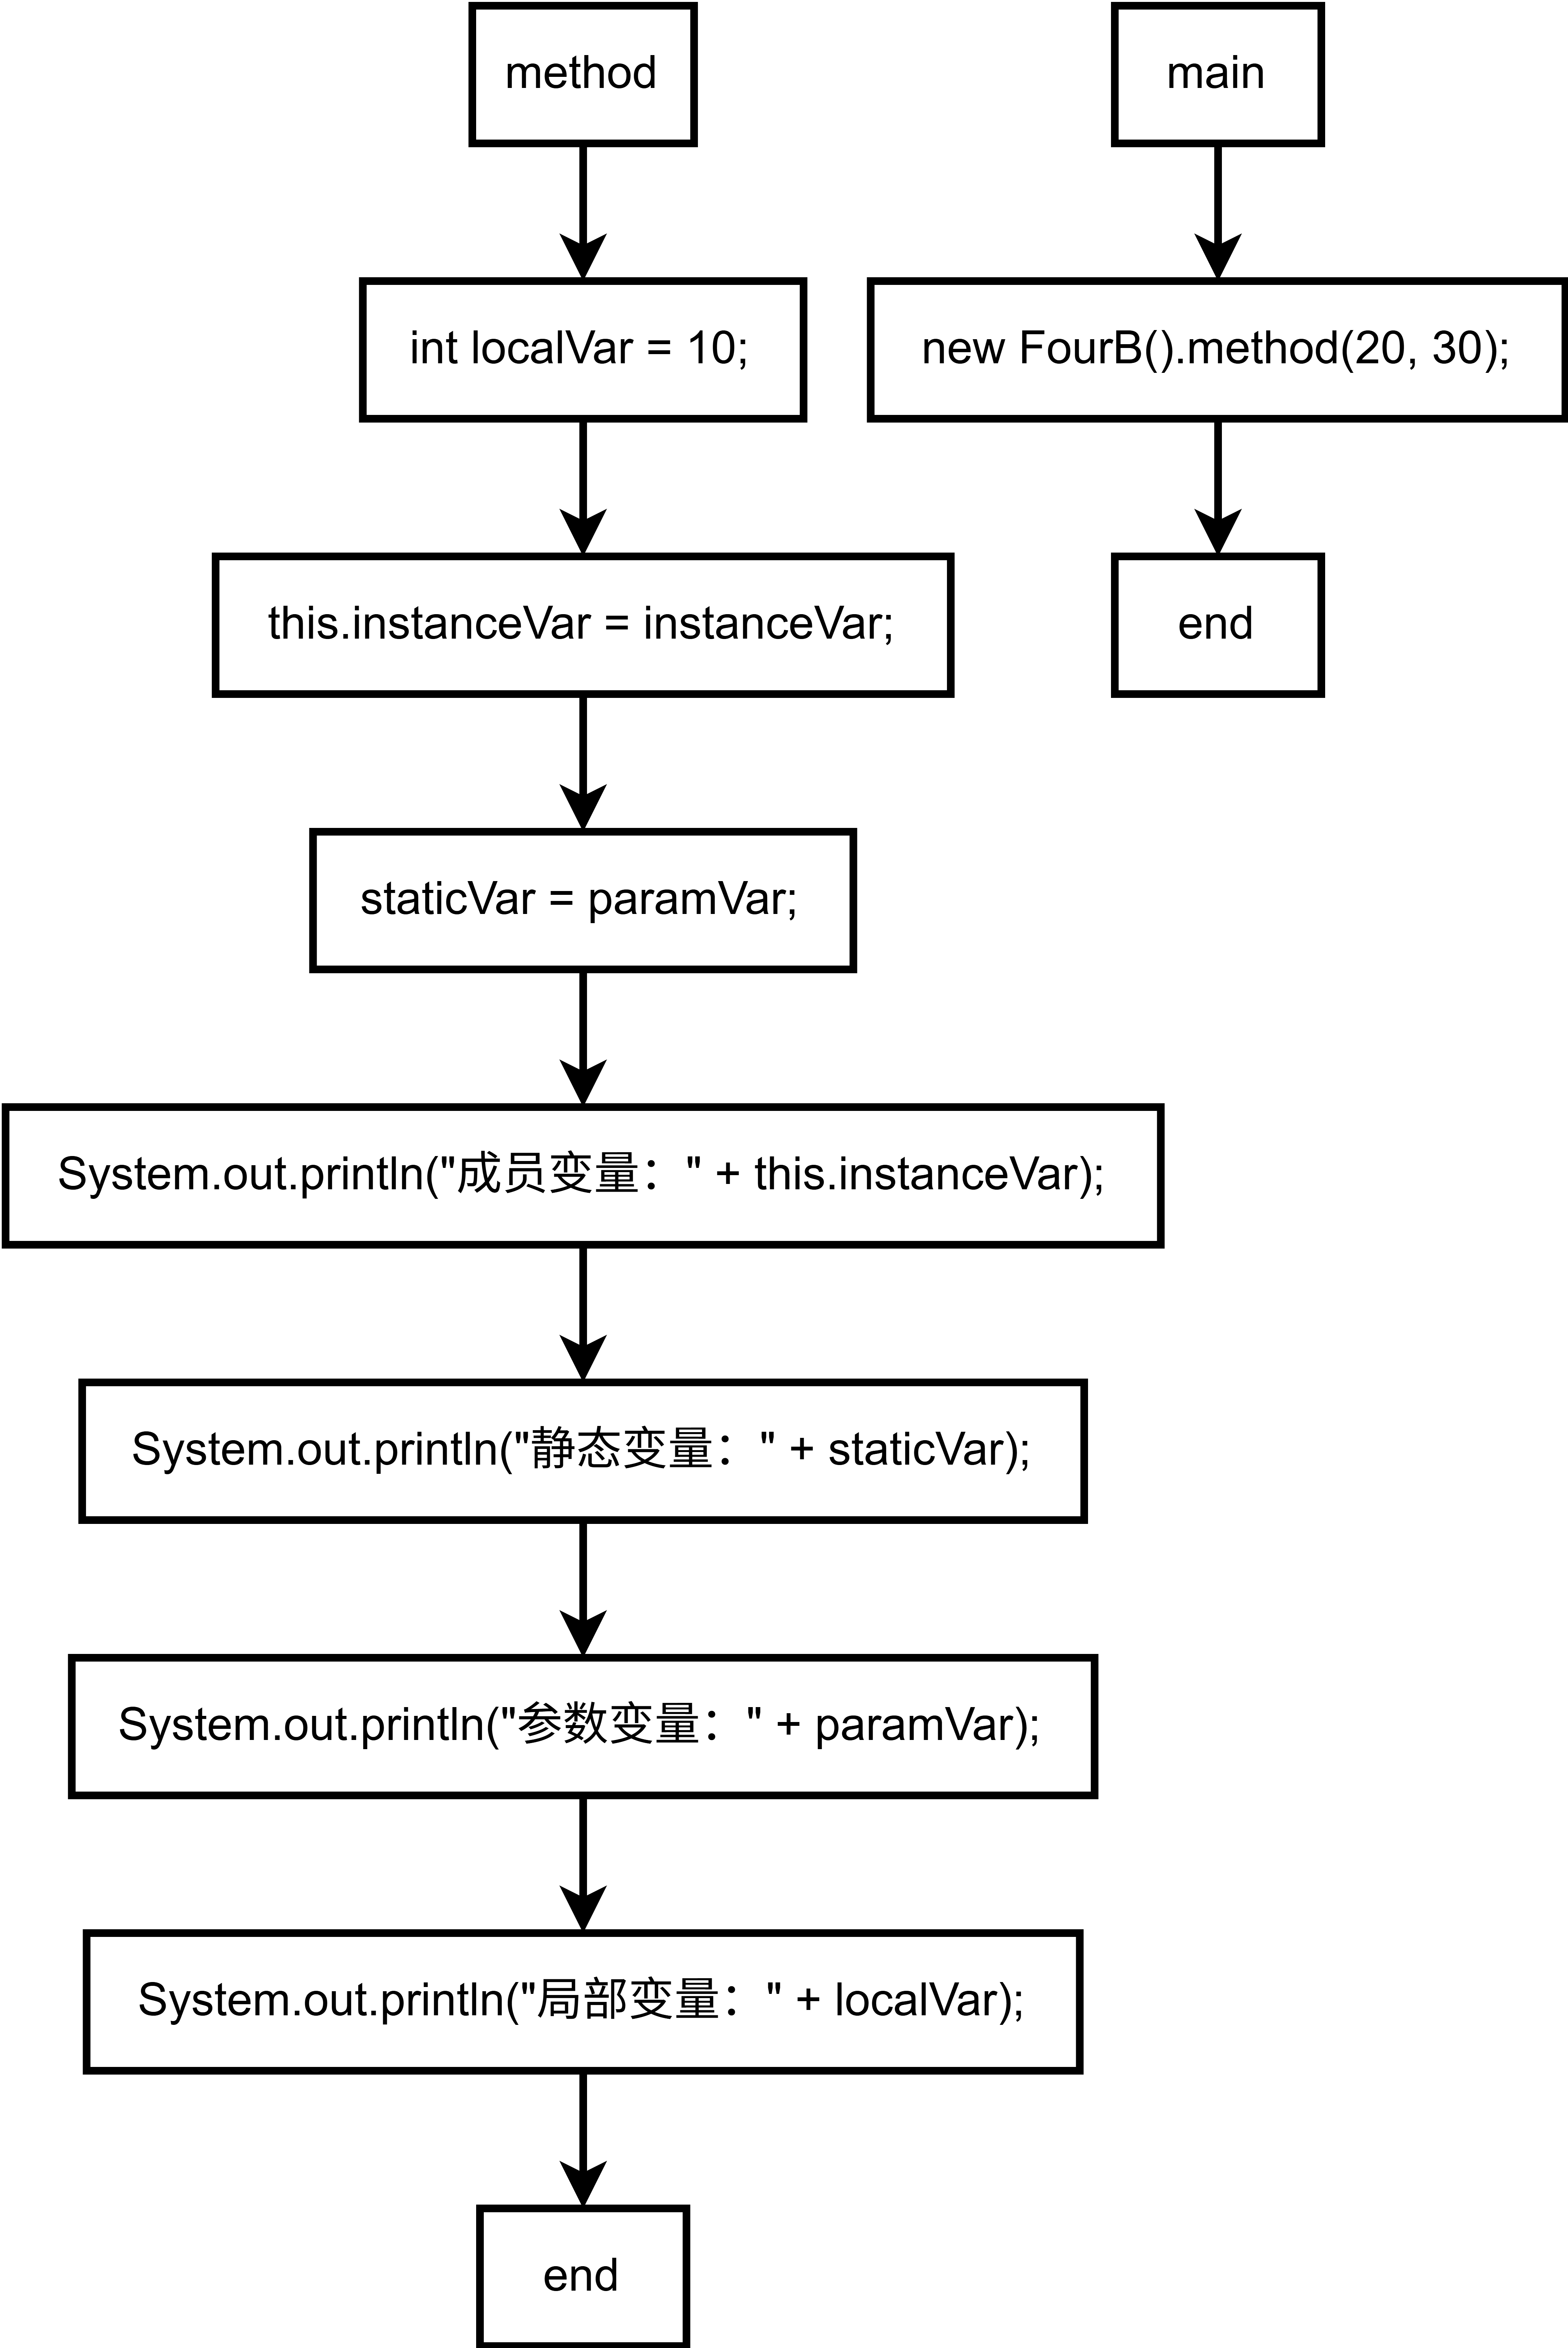
\includegraphics[width=0.8\textwidth]{fourb1.png}
\caption{流程图}
\end{figure}

\subsection*{源代码说明}
演示实例变量、静态变量与 this 的使用区别。实例方法通过 this 区分同名参数与成员变量,并输出实例变量、静态变量、参数及局部变量的值。主程序创建 FourB 实例并调用方法以展示变量作用域与赋值效果;点击查看\hyperref[sec:four]{Four.java完整代码}。

\subsection*{实验过程与结果}

\begin{figure}[H]
\centering
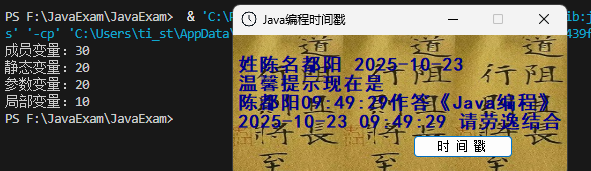
\includegraphics[width=0.8\textwidth]{fourb.png}
\caption{运行结果}
\end{figure}

\section*{【第五个实验具体内容】}
\subsection*{流程图}

\begin{figure}[H]
\centering
\includegraphics[width=0.8\textwidth]{fiveb1.png}
\caption{流程图}
\end{figure}

\subsection*{源代码说明}
定义抽象/接口驱动的形状体系(Shape/ IShapeArea),并由 Rectangle、Circle 与 Square 实现周长与面积计算。主程序通过多态遍历不同形状,打印各形状信息并累计总周长与总面积。代码用于练习继承、多态与代码复用;点击查看\hyperref[sec:five]{Five.java完整代码}。

\subsection*{实验过程与结果}

\begin{figure}[H]
\centering
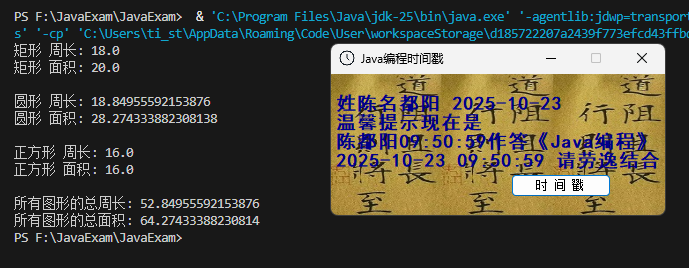
\includegraphics[width=0.8\textwidth]{fiveb.png}
\caption{运行结果}
\end{figure}

\section*{【第六个实验具体内容】}
\subsection*{流程图}

\begin{figure}[H]
\centering
\includegraphics[width=0.8\textwidth]{sixb1.png}
\caption{流程图}
\end{figure}

\subsection*{源代码说明}
练习继承与方法覆盖/重载的组合使用。父类 A 定义 sum1 与 sum2(int),子类 B 覆盖无参 sum2 并重载 sum2(int),且提供 sum3 通过 super 调用父类实现。主程序实例化子类并调用这些方法以演示不同调用路径与结果;点击查看\hyperref[sec:six]{Six.java完整代码}。

\subsection*{实验过程与结果}

\begin{figure}[H]
\centering
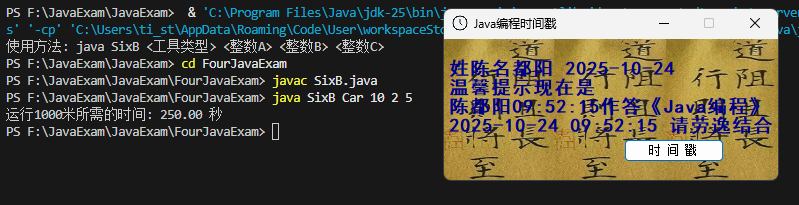
\includegraphics[width=0.8\textwidth]{sixb.png}
\caption{运行结果}
\end{figure}

\section*{【第七个实验具体内容】}
\subsection*{流程图}

\begin{figure}[H]
\centering
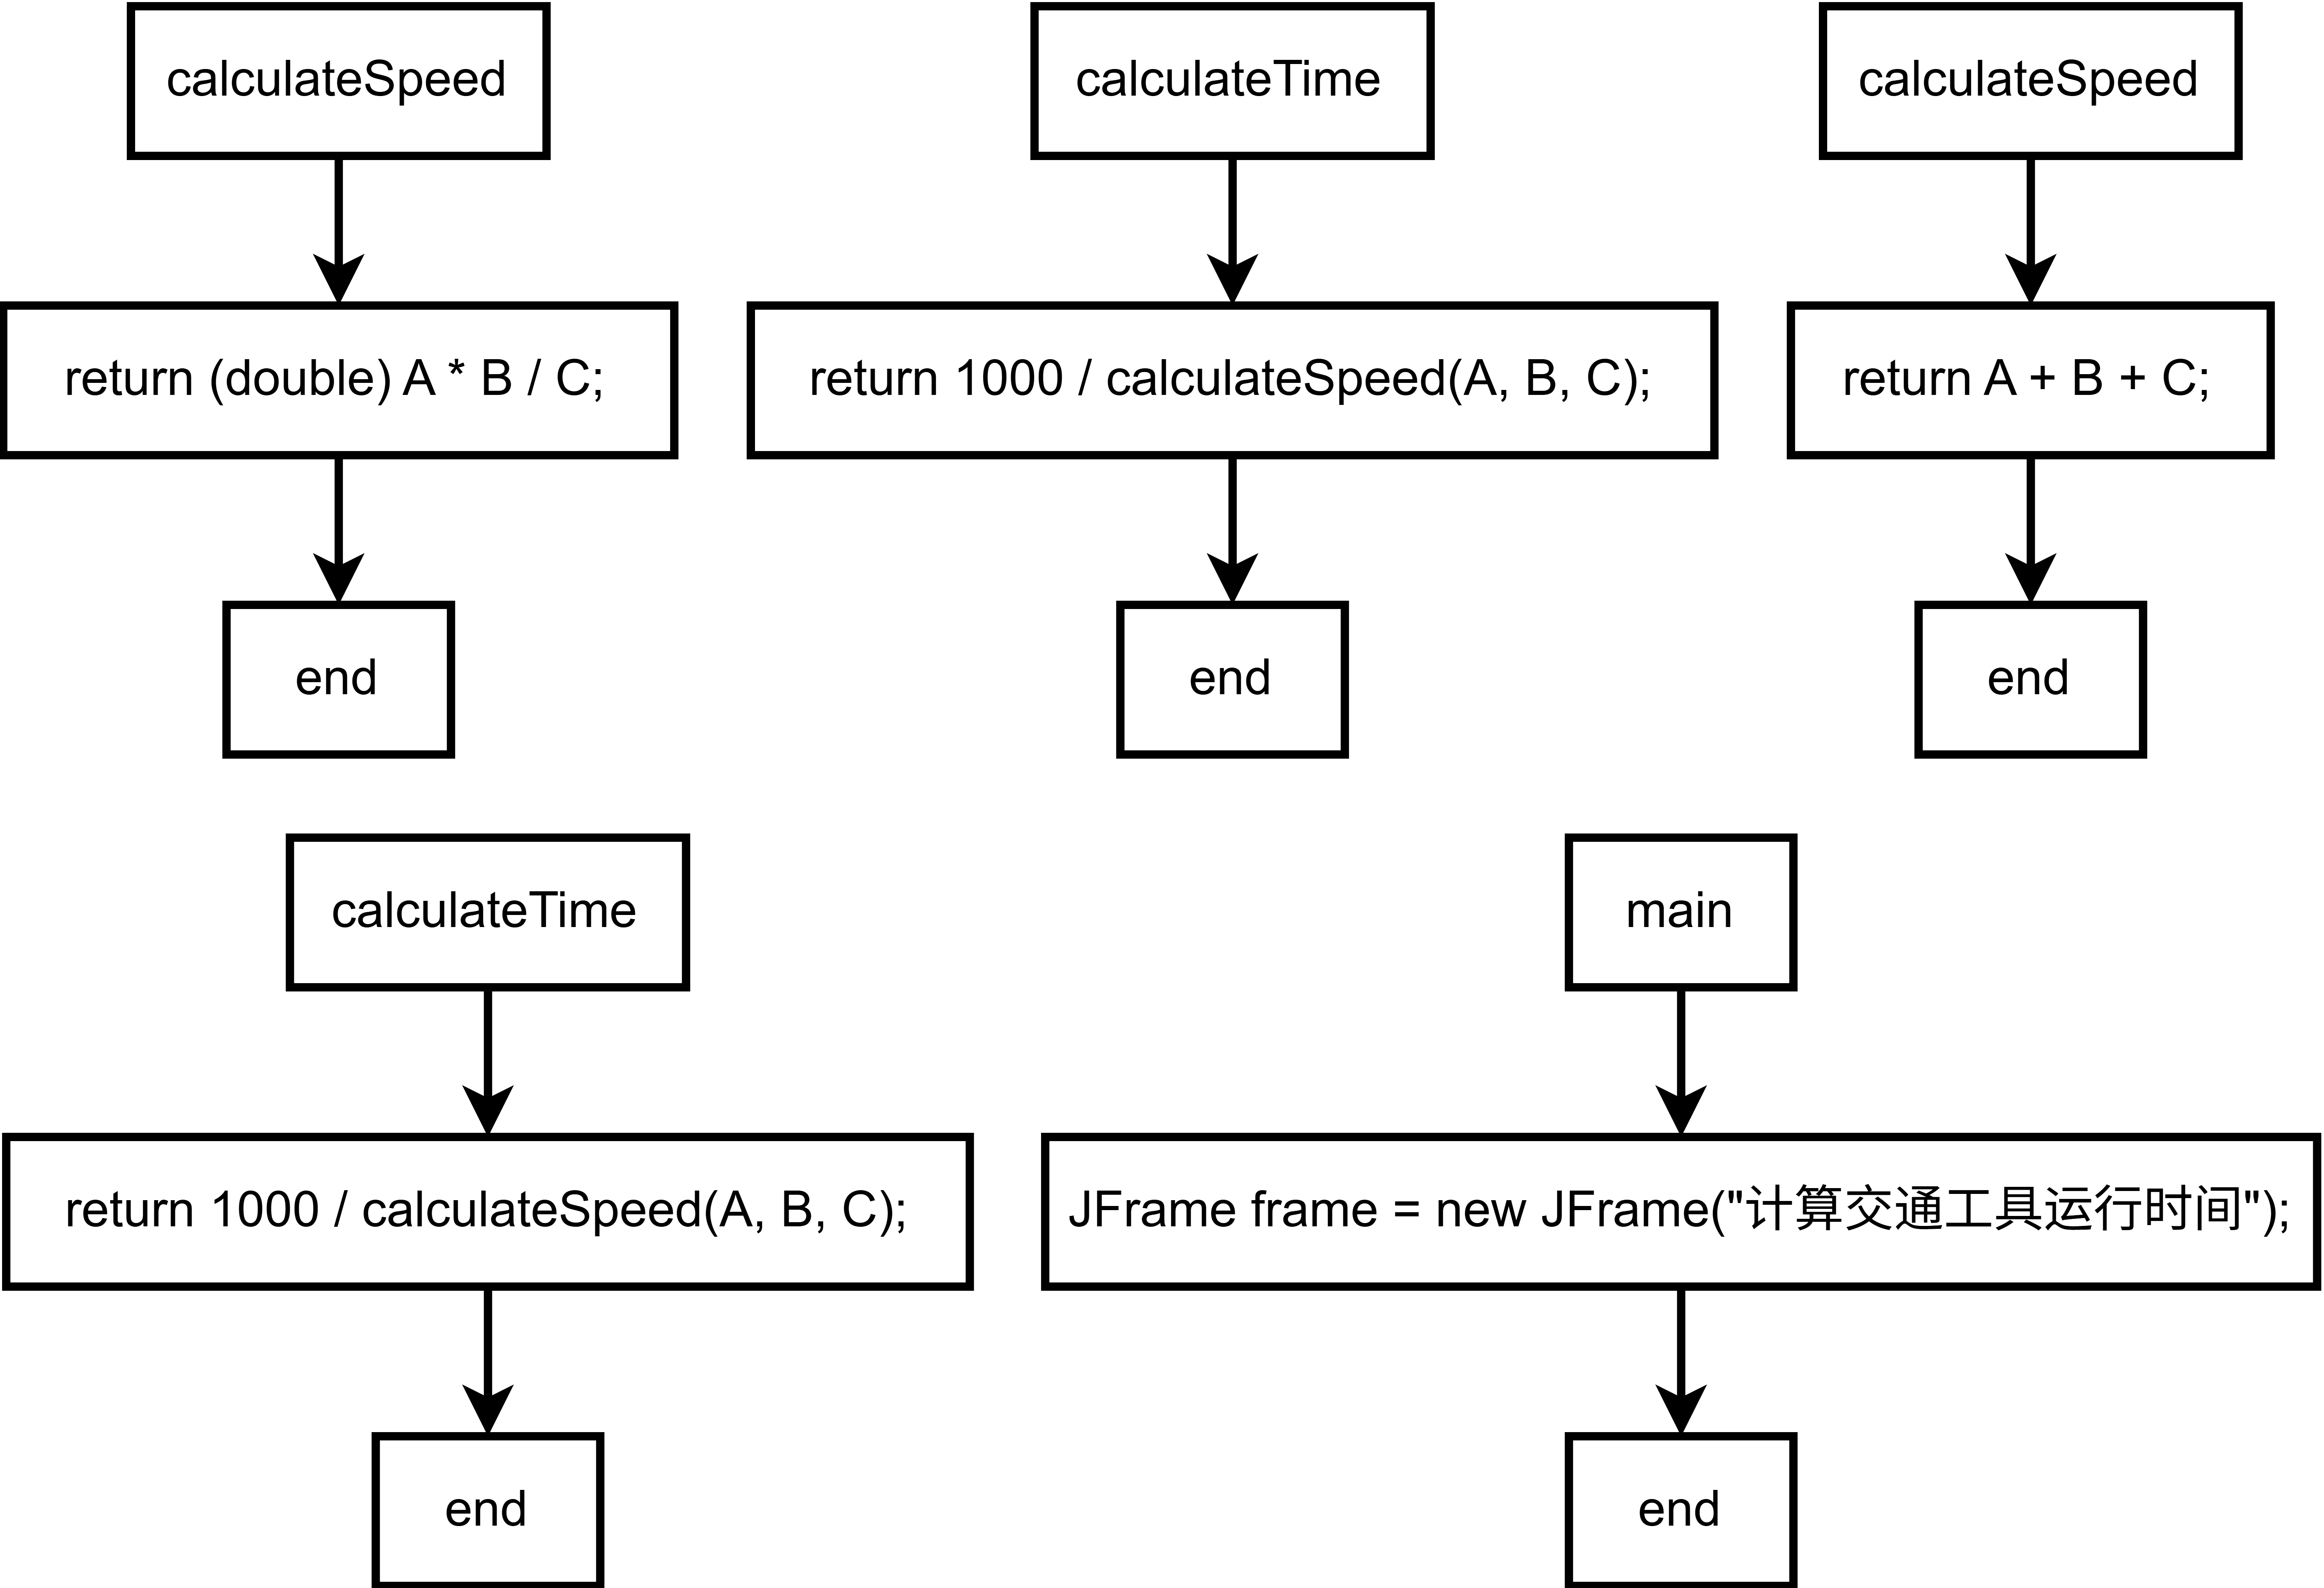
\includegraphics[width=0.8\textwidth]{sevenb1.png}
\caption{流程图}
\end{figure}

\subsection*{源代码说明}
基于 GUI 的反射与接口示例:定义接口 ICommon 及实现类(Car、Plane),并在界面中通过反射动态加载指定的车辆类。界面接收参数并计算旅行时间,结果显示在文本框,同时展示反射的特点与错误处理。主程序构建窗口并支持动态实例化与交互;点击查看\hyperref[sec:seven]{Seven.java完整代码}。


\subsection*{实验过程与结果}

\begin{figure}[H]
\centering
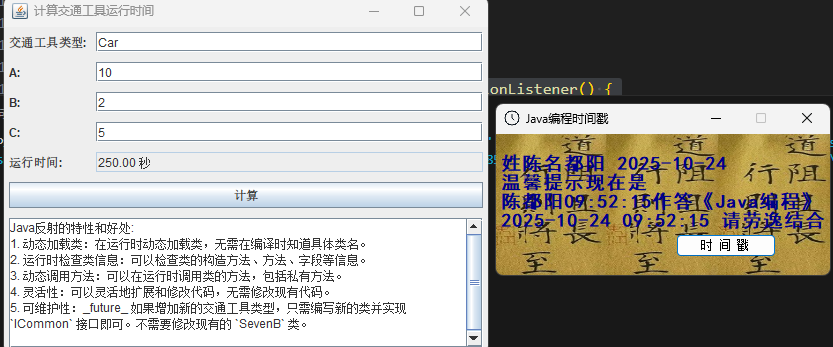
\includegraphics[width=0.8\textwidth]{sevenb.png}
\caption{运行结果}
\end{figure}



\section*{【实验心得】}
    本次实验主要花费时间在第六个实验上,其他实验都比较简单,主要是考察对基本算法的理解与实现。\\
    
    第六个实验我在思考Java反射可以突破封装,这就有些离谱,但是抽象的是,在linux平台上报错InaccessibleObjectException,这就很奇怪。暂时没解决\\

    但更抽象的是反射时获取不到实际泛型参数,这就很难受,而且直接获取其封装后的内容,这直接打破安全性哇。\\

    至于反射安全性这块,我觉得还是需要深入理解,毕竟这是一个很重要的区域。任何一家企业都会对安全性的权重较大。\\

    最后由于时间延长我如果在搓完A阻的万年历,可以拿C\#来写个seven的实验,直接加入一个可以直接添加新车的区域。\\
\newpage
\begin{center}
    {\zihao{1}\heiti 附录}
\end{center}
{\zihao{2}【代码附录】}\\

\section*{One.java源代码}\label{sec:one}
\begin{lstlisting}
// One.java
abstract class Shape {
    // Abstract method - calculate area
    abstract double area();
    
    // Abstract method - print area
    abstract void printArea();
}

class Rectangle extends Shape {
    private double width;
    private double height;
    
    public Rectangle(double width, double height) {
        this.width = width;
        this.height = height;
    }
    
    @Override
    double area() {
        return width * height;
    }
    
    @Override
    void printArea() {
        System.out.println("The area of the rectangle is: " + area());
    }
}

class Circle extends Shape {
    private double radius;
    
    public Circle(double radius) {
        this.radius = radius;
    }
    
    @Override
    double area() {
        return Math.PI * radius * radius;
    }
    
    @Override
    void printArea() {
        System.out.println("The area of the circle is: " + area());
    }
}

// Main class
public class OneB {
    public static void main(String[] args) {
        // Create a rectangle object
        Shape rect = new Rectangle(5, 4);
        rect.printArea();
        
        // Create a circle object
        Shape circle = new Circle(3);
        circle.printArea();
    }
}

\end{lstlisting}

\section*{Two.java源代码}\label{sec:two}
\begin{lstlisting}
// TwoA.java
// Parent class A
class A {
    int sum, num1, num2;
    
    public A() {
        num1 = 10;
        num2 = 20;
        sum = 0;
    }
    
    // Method sum1 - calculate num1 + num2
    void sum1() {
        sum = num1 + num2;
        System.out.println("sum=" + num1 + "+" + num2 + "=" + sum);
    }
    
    // Method sum2 - overloaded method with one parameter n
    void sum2(int n) {
        num1 = n;
        sum = num1 + num2;
        System.out.println("sum=" + num1 + "+" + num2 + "=" + sum);
    }
}

// Subclass B - inherits from A
class B extends A {
    int num2;  
    
    public B() {
        num2 = 200; 
    }
    
    // sum2 method - overrides the parent class method sum2()
    void sum2() {
        sum = num1 + num2;
        System.out.println("sum=" + num1 + "+" + num2 + "=" + sum);
    }
    
    // sum2 method - overloaded method with one parameter n
    void sum2(int n) {
        num1 = n;
        sum = num1 + num2;
        System.out.println("sum=" + num1 + "+" + num2 + "=" + sum);
    }
    

    void sum3(int n) {
        super.sum2(n);  // Call parent class's sum2(int n) method
        System.out.println("sum=" + num1 + "=" + sum);
    }
}

// Test class
public class TwoB {
    public static void main(String[] arg) {
        B m = new B();
        m.sum1();      // Calls inherited sum1() method from class A
        m.sum2();      // Calls overridden sum2() method in class B (no parameters)
        m.sum2(50);    // Calls overloaded sum2(int n) method in class B
        m.sum3(50);    // Calls sum3(int n) method in class B
    }
}

\end{lstlisting}

\section*{Three.java源代码}\label{sec:three}
\begin{lstlisting}
// Three.java
import java.io.*;

// Parent class - SuperClass
class SuperClass {
    int x;
    
    // Constructor of the parent class
    SuperClass() {
        x = 3;
        System.out.println("in SuperClass : x=" + x);
    }
    
    // Method of the parent class
    void doSomething() {
        System.out.println("in SuperClass.doSomething()");
    }
}

// Child class - SubClass, inherits from SuperClass
class SubClass extends SuperClass {
    int x;  
    
    // Constructor of the child class
    SubClass() {
        super();  // Call the parent class constructor
        x = 5;    // Initialize the subclass variable
        System.out.println("in SubClass : x=" + x);
    }
    
    // Overriding the parent class method
    void doSomething() {
        super.doSomething();  // Call the parent version of doSomething()
        System.out.println("in SubClass.doSomething()");
        System.out.println("super.x=" + super.x + " sub.x=" + x);
    }
}

public class ThreeB {
    
    public static void main(String[] args) { 
        // Create a SubClass object
        SubClass subC = new SubClass();
        
        System.out.println();
        
        // Call the method of the object
        subC.doSomething();
    }
}

\end{lstlisting}

\section*{Four.java源代码}\label{sec:four}
\begin{lstlisting}
// Four.java
public class FourB {
    // Instance variable
    private int instanceVar;

    // Static variable
    private static int staticVar;

    // Instance method (removed static modifier to allow use of 'this')
    public void method(int paramVar, int instanceVar) {
        // Local variable
        int localVar = 10;

        // Variable assignment
        this.instanceVar = instanceVar; // Use 'this' to distinguish member variable and parameter variable
        staticVar = paramVar;

        System.out.println("Instance variable: " + this.instanceVar);
        System.out.println("Static variable: " + staticVar);
        System.out.println("Parameter variable: " + paramVar);
        System.out.println("Local variable: " + localVar);
    }

    public static void main(String[] args) {
        // Create an instance and call the method
        new FourB().method(20, 30);
    }
}

\end{lstlisting}

\section*{Five.java源代码}\label{sec:five}
\begin{lstlisting}
// Five.java
// Define interface IShapeArea
interface IShapeArea {
    double getArea();
}

// Abstract class Shape
abstract class Shape implements IShapeArea {
    protected String name;
    
    public Shape(String name) {
        this.name = name;
    }
    
    // Abstract method: calculate perimeter
    public abstract double getPerimeter();
    
    // Common method: print information
    public void printInfo() {
        System.out.println(name + " Perimeter: " + getPerimeter());
        System.out.println(name + " Area: " + getArea());
    }
}

// Rectangle class
class Rectangle extends Shape {
    private double width;
    private double height;

    public Rectangle(double width, double height) {
        super("Rectangle");
        this.width = width;
        this.height = height;
    }

    @Override
    public double getPerimeter() {
        return 2 * (width + height);
    }

    @Override
    public double getArea() {
        return width * height;
    }

    // Public getter methods
    public double getWidth() {
        return width;
    }

    public double getHeight() {
        return height;
    }
}

// Circle class
class Circle extends Shape {
    private double radius;

    public Circle(double radius) {
        super("Circle");
        this.radius = radius;
    }

    @Override
    public double getPerimeter() {
        return 2 * Math.PI * radius;
    }

    @Override
    public double getArea() {
        return Math.PI * radius * radius;
    }
}

// Square class, inherits from Rectangle
class Square extends Rectangle {
    public Square(double side) {
        super(side, side);
        this.name = "Square";
    }

    @Override
    public double getPerimeter() {
        return 4 * super.getWidth();
    }

    @Override
    public double getArea() {
        return super.getWidth() * super.getWidth();
    }
}

public class FiveB {
    public static void main(String[] args) {
        // Use polymorphism to handle different shapes
        Shape[] shapes = {
            new Rectangle(5, 4),
            new Circle(3),
            new Square(4)
        };

        double totalPerimeter = 0;
        double totalArea = 0;

        // Process all shapes uniformly
        for (Shape shape : shapes) {
            shape.printInfo();
            totalPerimeter += shape.getPerimeter();
            totalArea += shape.getArea();
            System.out.println();
        }

        System.out.println("Total Perimeter of all shapes: " + totalPerimeter);
        System.out.println("Total Area of all shapes: " + totalArea);
    }
}

\end{lstlisting}

\section*{Six.java源代码}\label{sec:six}
\begin{lstlisting}
// Six.java
// Superclass A
class A {
    int sum, num1, num2;
    
    public A() {
        num1 = 10;
        num2 = 20;
        sum = 0;
    }
    
    // Method sum1 - calculate num1 + num2
    void sum1() {
        sum = num1 + num2;
        System.out.println("sum=" + num1 + "+" + num2 + "=" + sum);
    }
    
    // Method sum2 - overloaded method, receives one parameter n
    void sum2(int n) {
        num1 = n;
        sum = num1 + num2;
        System.out.println("sum=" + num1 + "+" + num2 + "=" + sum);
    }
}

// Subclass B - extends A
class B extends A {
    int num2;  
    
    public B() {
        num2 = 200; 
    }
    
    // sum2 method - override superclass sum2 method
    void sum2() {
        sum = num1 + num2;
        System.out.println("sum=" + num1 + "+" + num2 + "=" + sum);
    }
    
    // sum2 method - overloaded, receives one parameter n
    void sum2(int n) {
        num1 = n;
        sum = num1 + num2;
        System.out.println("sum=" + num1 + "+" + num2 + "=" + sum);
    }
    
    // sum3 method - new method, calls superclass sum2
    void sum3(int n) {
        super.sum2(n);  // call superclass's sum2(int n)
        System.out.println("sum=" + num1 + "=" + sum);
    }
}

// Test class
public class TwoB {
    public static void main(String[] arg) {
        B m = new B();
        m.sum1();      // call inherited sum1 method from superclass A
        m.sum2();      // call newly defined sum2() method in subclass B (no param)
        m.sum2(50);    // call sum2(int n) method in subclass B
        m.sum3(50);    // call sum3(int n) method in subclass B
    }
}


\end{lstlisting}

\section*{Seven.java源代码}\label{sec:seven}
\begin{lstlisting}
// Seven.java
import java.awt.*;
import java.awt.event.ActionEvent;
import java.awt.event.ActionListener;
import java.lang.reflect.Constructor;
import javax.swing.*;

// Define interface ICommon
interface ICommon {
    double calculateSpeed(int A, int B, int C);
    double calculateTime(int A, int B, int C);
}

// Implement Car class
class Car implements ICommon {
    @Override
    public double calculateSpeed(int A, int B, int C) {
        return (double) A * B / C;
    }

    @Override
    public double calculateTime(int A, int B, int C) {
        return 1000 / calculateSpeed(A, B, C);
    }
}

// Implement Plane class
class Plane implements ICommon {
    @Override
    public double calculateSpeed(int A, int B, int C) {
        return A + B + C;
    }

    @Override
    public double calculateTime(int A, int B, int C) {
        return 1000 / calculateSpeed(A, B, C);
    }
}

// SevenB class using reflection
public class SevenB {
    public static void main(String[] args) {
        // Create GUI window
        JFrame frame = new JFrame("Calculate Vehicle Travel Time");
        frame.setDefaultCloseOperation(JFrame.EXIT_ON_CLOSE);
        frame.setSize(500, 350);
        frame.setLayout(new GridBagLayout());

        // Create GridBagConstraints
        GridBagConstraints gbc = new GridBagConstraints();
        gbc.insets = new Insets(5, 5, 5, 5); // Set spacing between components
        gbc.fill = GridBagConstraints.HORIZONTAL; // Fill horizontally
        gbc.anchor = GridBagConstraints.WEST; // Align components to the left

        // Add labels and input fields
        JLabel vehicleLabel = new JLabel("Vehicle Type:");
        gbc.gridx = 0;
        gbc.gridy = 0;
        frame.add(vehicleLabel, gbc);

        JTextField vehicleField = new JTextField();
        gbc.gridx = 1;
        gbc.gridy = 0;
        frame.add(vehicleField, gbc);

        JLabel ALabel = new JLabel("A:");
        gbc.gridx = 0;
        gbc.gridy = 1;
        frame.add(ALabel, gbc);

        JTextField AField = new JTextField();
        gbc.gridx = 1;
        gbc.gridy = 1;
        frame.add(AField, gbc);

        JLabel BLabel = new JLabel("B:");
        gbc.gridx = 0;
        gbc.gridy = 2;
        frame.add(BLabel, gbc);

        JTextField BField = new JTextField();
        gbc.gridx = 1;
        gbc.gridy = 2;
        frame.add(BField, gbc);

        JLabel CLabel = new JLabel("C:");
        gbc.gridx = 0;
        gbc.gridy = 3;
        frame.add(CLabel, gbc);

        JTextField CField = new JTextField();
        gbc.gridx = 1;
        gbc.gridy = 3;
        frame.add(CField, gbc);

        JLabel resultLabel = new JLabel("Travel Time:");
        gbc.gridx = 0;
        gbc.gridy = 4;
        frame.add(resultLabel, gbc);

        JTextField resultField = new JTextField();
        resultField.setEditable(false);
        gbc.gridx = 1;
        gbc.gridy = 4;
        frame.add(resultField, gbc);

        // Add calculate button
        JButton calculateButton = new JButton("Calculate");
        gbc.gridx = 0;
        gbc.gridy = 5;
        gbc.gridwidth = 2; // Span two columns
        gbc.anchor = GridBagConstraints.CENTER; // Center the button
        frame.add(calculateButton, gbc);

        // Add text area to show reflection features and benefits
        JTextArea reflectionInfo = new JTextArea();
        reflectionInfo.setEditable(false);
        reflectionInfo.setLineWrap(true);
        reflectionInfo.setWrapStyleWord(true);
        JScrollPane scrollPane = new JScrollPane(reflectionInfo);

        String infoText = "Features and Benefits of Java Reflection:\n"
                        + "1. Dynamic class loading: Load classes at runtime without knowing class names at compile time.\n"
                        + "2. Inspect class information at runtime: Access constructors, methods, fields, etc.\n"
                        + "3. Dynamic method invocation: Call class methods at runtime, including private methods.\n"
                        + "4. Flexibility: Extend and modify code without changing existing code.\n"
                        + "5. Maintainability: In the future, adding a new vehicle type only requires creating a new class implementing the `ICommon` interface, without modifying the existing `SevenB` class.\n";

        reflectionInfo.setText(infoText);
        gbc.gridx = 0;
        gbc.gridy = 6;
        gbc.gridwidth = 2; // Span two columns
        gbc.fill = GridBagConstraints.BOTH; // Fill entire area
        gbc.weightx = 1.0;
        gbc.weighty = 1.0;
        frame.add(scrollPane, gbc);

        // Button click event handler
        calculateButton.addActionListener(new ActionListener() {
            @Override
            public void actionPerformed(ActionEvent e) {
                String vehicleType = vehicleField.getText();
                try {
                    int A = Integer.parseInt(AField.getText());
                    int B = Integer.parseInt(BField.getText());
                    int C = Integer.parseInt(CField.getText());

                    // Create instance using reflection
                    Class<?> clazz = Class.forName(vehicleType);
                    Constructor<?> constructor = clazz.getDeclaredConstructor();
                    ICommon vehicle = (ICommon) constructor.newInstance();

                    // Calculate and display time, rounded to 2 decimal places
                    double time = vehicle.calculateTime(A, B, C);
                    resultField.setText(String.format("%.2f seconds", time));
                } catch (ClassNotFoundException ex) {
                    JOptionPane.showMessageDialog(frame, "Vehicle type not found: " + vehicleType, "Error", JOptionPane.ERROR_MESSAGE);
                } catch (NumberFormatException ex) {
                    JOptionPane.showMessageDialog(frame, "Please enter valid integers", "Error", JOptionPane.ERROR_MESSAGE);
                } catch (Exception ex) {
                    ex.printStackTrace();
                    JOptionPane.showMessageDialog(frame, "Error creating vehicle instance", "Error", JOptionPane.ERROR_MESSAGE);
                }
            }
        });

        // Show the window
        frame.setVisible(true);
    }
}


\end{lstlisting}

\end{document}

